\subsection{M.PC.7 - Variazione del piano tra preventivo e consuntivo}
\begin{figure}[H]
    \centering
    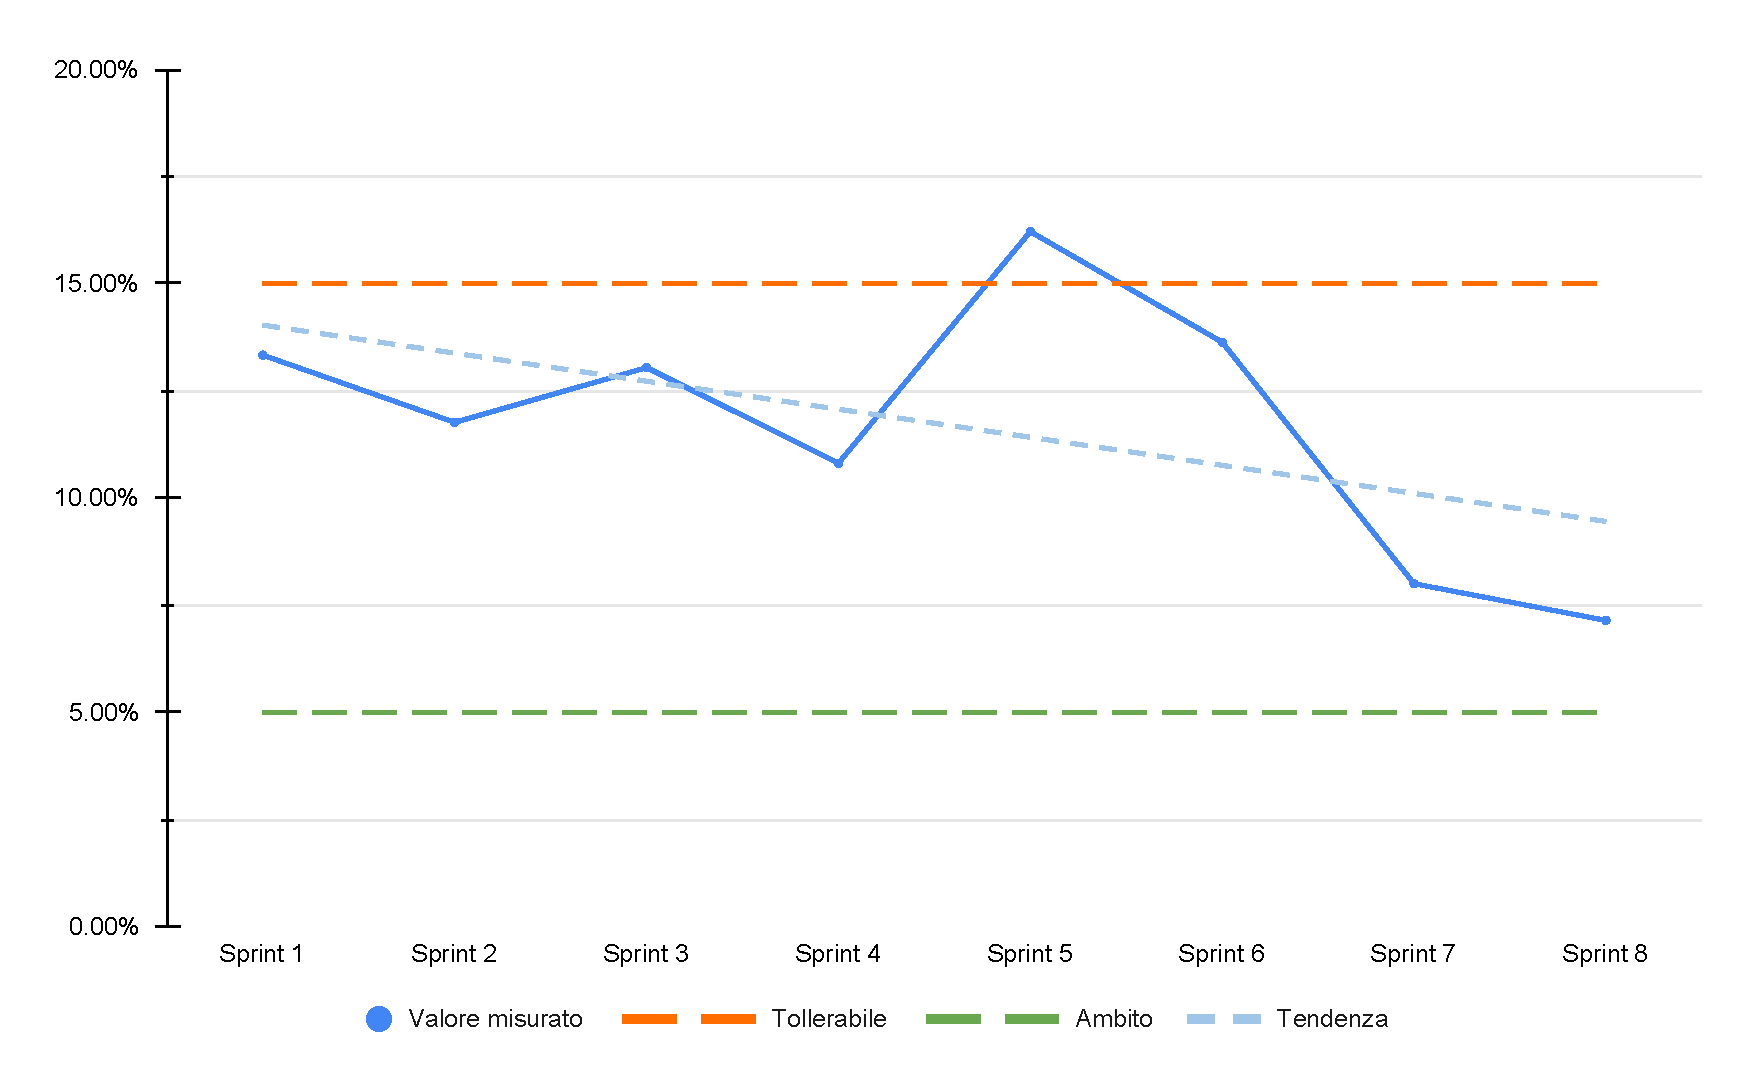
\includegraphics[width=\textwidth]{assets/variazione_task_completati.pdf}
    \caption{M.PC.7 - Variazione del piano tra preventivo e consuntivo}
\end{figure}

\par Il gruppo ha mantenuto un sano equilibrio nel rapporto tra le attività pianificate ad inizio \glossario{sprint} e quelle non portate a termine all'interno del periodo determinato. Il risultato è indice di una pianificazione iniziale discretamente accurata, anche se non ottimale. Il picco in corrispondenza dello \glossario{sprint} 5 è dovuto alla sua durata minore, per cui la pianificazione iniziale non è stata bilanciata adeguatamente. A partire dalla misura successiva si è tuttavia riconsiderato il carico di lavoro, rientrando nel range di tollerabilità.